\documentclass[12pt,aspectratio=169]{beamer}

\usetheme[progressbar=frametitle, numbering=fraction]{metropolis}
\usepackage{appendixnumberbeamer}
\usepackage{gensymb}
\usepackage{booktabs}
\usepackage[scale=2]{ccicons}

\usepackage{pgfplots}
\usepgfplotslibrary{dateplot}
% \usepackage[english]{babel}
\usepackage{babel}

\usepackage{xspace}
\newcommand{\themename}{\textbf{\textsc{metropolis}}\xspace}

% Chinese Fonts (Fontset: fandol,ubuntu)
\usepackage[fontset=fandol]{ctex}

% Math Fonts
\usefonttheme{professionalfonts} 
\usepackage{mathspec}
\setsansfont[BoldFont={Fira Sans},
Numbers={OldStyle}]{Fira Sans Light}
\setmathsfont(Digits)[Numbers={Lining, Proportional}]{Fira Sans Light}

% Change Color of the theme
\usepackage{xcolor}
\definecolor{DarkGrey}{HTML}{353535}
\definecolor{ECNURed}{RGB}{164,31,53}
\definecolor{ECNUBrown}{RGB}{134,117,77}
\definecolor{BackGround}{RGB}{250,250,250}
\definecolor{MyBlue}{RGB}{0,161,233}
\definecolor{MyRed}{RGB}{228,0,127}
\setbeamercolor{normal text}{ fg= DarkGrey  }
\setbeamercolor{alerted text}{ fg= ECNURed  }
\setbeamercolor{example text}{ fg= ECNUBrown  }

% Bolder Fonts for presenting in a large room 
\setsansfont[BoldFont={Fira Sans SemiBold}]{Fira Sans}
\metroset{block=fill}

\usepackage{listings,xcolor}
\usepackage{tikz}
\usepackage{pgfmath}
\usepackage{animate,media9,graphicx}
\usepackage{subcaption}
\usepackage{calligra}
\usepackage{array}
\renewcommand{\arraystretch}{2}  % 增加行高
\setlength{\tabcolsep}{10pt}       % 增加列间距

\usepackage[backend=biber,style=gb7714-2015,sorting=none]{biblatex}
\setbeamerfont{bibliography item}{size=\tiny}
\setbeamerfont{bibliography entry author}{size=\tiny}
\setbeamerfont{bibliography entry title}{size=\tiny}
\setbeamerfont{bibliography entry location}{size=\tiny}
\setbeamerfont{bibliography entry note}{size=\tiny}
\renewcommand{\bibfont}{\tiny}
\addbibresource{slides.bib}

\lstset{
	language         = c++,
	numbers          = left,
	numberstyle      = \tiny,
	breaklines       = true,
	captionpos       = b,
	tabsize          = 4,
	frame            = shadowbox,
	columns          = fullflexible,
	commentstyle     = \color[RGB]{0,128,0},
	keywordstyle     = \color[RGB]{0,0,255},
	basicstyle       = \tiny\ttfamily,
	stringstyle      = \color[RGB]{148,0,209}\ttfamily,
	rulesepcolor     = \color{red!20!green!20!blue!20},
	showstringspaces = false,
}

\title{基于蒙特卡洛树搜索的等面积划分球面中周长极小值探索}
% \subtitle{}
\date{\today}
\author{汇报人:丁逸飞\ \ \ \ \ \ \ \ \ \ 指导老师:王二小}
% \institute{}
% \titlegraphic{\hfill
\includegraphics[height=1.5cm]{ECNUlogo.png}}

\begin{document}

\maketitle
\footnotesize
\begin{frame}{Contents}
  \setbeamertemplate{section in toc}[sections numbered]
  \tableofcontents%[hideallsubsections]
\end{frame}

\section{选题背景与意义}

\begin{frame}{选题背景与意义}

  \begin{block}{蜂巢问题}

    构造一个平面的等面积划分,使得这个划分的总周长尽可能的小. 

  \end{block}

  1999 年,Hales\cite{hales2001honeycomb}证明了最优解为平面的正六边形密铺,同时将其平面上的理论应用到了球
  面之上,证明了对于 $n = 12$ 的球面蜂巢问题,正五边形分割的总周长是最小的. 此后,人
  们相继证明了 $n = 2, 3, 4, 6$ 的几种情况,其他情况都还等待着我们去发现. 

  通过研究球面蜂巢问题,我们既可以深入探索几何排列问题,寻找更一般的排列规律和方
  法,也可以深入探索空间优化理论和方法,对于工程、建筑和计算机图形学等领域的空间布
  局和规划具有非常重要的理论意义. 

\end{frame}

\section{文献综述}

\begin{frame}{经典蜂巢问题研究进展}

  蜂巢问题寻求将平面划分为单位区域的最小周长方法,经过长期推测,蜂巢定理指出,正六
  边形提供了这种最小周长的划分,并由 Hales 于 1999 年证明\cite{hales2001honeycomb}. 对于球体的类似猜测是划
  分为 $n$ 个全等的正 $m$ 边形可以使划分为 $n$ 个相等区域的周长最小化,事实上,只存在五种
  这样的分区. 

  后来,Hales 推广了他的平面方法来证明 $n = 12$ 的情况,即 $12$ 个正五边形的十二面体排列
  为周长最小的情况. 1994 年,Masters\cite{masters1996perimeter}使用肥皂泡理论工具和计算机论证证明了球体上的
  双泡定理,等效解决了 $n = 3$ 时的球面蜂巢问题. 2007 年,Conor Quinn\cite{quinn2007least}为Masters 的结
  果提供了新的证明,并且处理了 $n = 4$ 的情况. 2010 年,Cox 和Flikkema\cite{cox2010minimal}利用数学软件
  计算了 $n \leq 42$ 的候选情况. 目前还没有利用启发式搜索求解该问题的论文. 

\end{frame}

\begin{frame}{球面离散划分的现有方法}

  \begin{itemize}

    \item 几何对称法:此类方法的局限性在于仅适用于满足 $N=12,4,6$ 
    等特定数值的情形(对应正多面体顶点数),且要求区域严格全等,该方法无法推广到非对称情形. 

    \item 变分法框架:Masters\cite{masters1996perimeter}得出结论:由三个具有恒定曲率的弧组成,
    在两个顶点处以 $120\degree$ 的角度相交,是围住两个区域的最短围栏. 
    证明两个相交大圆构成 $N=2$ 时的最优解. Quinn\cite{quinn2007least}扩展该框架至 $N=3$,
    这类方法的计算复杂度随 $N$ 增加呈指数增长,目前仅适用于 $N\leq4$ 的情形. 

    \item 计算几何法:Manuel等人\cite{caroli2010robust}提出球面Voronoi算法,提出了两种构建球面Delaunay三角剖分的方法. 
    Voronoi剖分技术在球面划分中展现出独特优势,为启发式搜索算法(如MCTS)的应用提供了理论突破口

  \end{itemize}

\end{frame}

\begin{frame}{MCTS在连续问题领域的应用案例}

  近年来,蒙特卡洛树搜索(MCTS)在连续优化领域取得突破性进展,其核心价值体现在高维空间中的智能探索与开发平衡机制. 

  \begin{itemize}

    \item 连续动作空间中的梯度优化:Lee等人\cite{lee2020monte}在AAAI 2020提出了VG-UCT算法,
    将蒙特卡洛树搜索(MCTS)与基于价值梯度的局部优化相结合,以解决连续动作空间中的规划问题. 

    \item 动态系统参数识别:Michelucci等人\cite{michelucci2024improving}将GRAVE启发式算法扩展到连续领域,
    提出了连续GRAVE(cGRAVE)方法,通过高斯卷积平滑来优化动作和状态值的估计. 

    \item 多目标连续优化:Wang等人\cite{wang2012multi}在ACML 2012提出的多目标MCTS框架,在MO-MCTS中,
    采用了超体积指标(hyper-volume indicator)来代替传统的UCB准则,以应对多维度奖励的优化问题. 

    \item 可学习的连续空间搜索:Lei等人\cite{lei2021kb}在IEEE 2021提出了一种新的可学习的连续蒙特卡罗树搜索方法,
    称为KB-Tree,用于自动驾驶中的运动规划. 

  \end{itemize}

\end{frame}

\section{数学基础与问题建模}

\begin{frame}{球面几何特征}

  测地线长度计算

  $$
    \begin{aligned}
      d&=r\times \arccos(\sin\phi_1\sin\phi_2\cos\Delta\lambda+\cos\phi_1\cos\phi_2)\\
      d&=2r\times \arctan(\sqrt{a},\sqrt{1-a}), a=\sin^2\frac{\Delta\phi}{2}+\cos\phi_1\cos\phi_2
      \sin^2\frac{\Delta\lambda}{2}
    \end{aligned}
  $$

  球面三角形面积公式

  $$
    \cos\alpha=\frac{\cos\theta_{BC}-\cos\theta_{AB}\cos\theta_{CA}}{\sin\theta_{AB}\sin\theta_{CA}},
    S=R^2\cdot(\alpha+\beta+\gamma-\pi)
  $$

\end{frame}

\begin{frame}{优化问题形式化}

  \begin{block}{问题描述}

    给定单位球面 $S^2\subset \mathbb{R}^2$,找到 $N$ 个互不重叠的连通区域 $\{\Omega_i\}_{i=1}^N$ 满足:
    \begin{itemize}
      \item 面积均等:$\forall i,\mu(\Omega_i)=\frac{4\pi}{N}$;
      \item 边界极小:总测地周长 $L_{total}=\sum\limits_{i=1}^Nl(\partial\Omega_i)$ 最小化;
      \item 完全覆盖:$\bigcup\limits_{i=1}^N\Omega_i=S^2$。
    \end{itemize}

  \end{block}

  建立最小化目标:
  $\min\limits_PJ(P)=\sum\limits_{i=1}^Nl(\partial\Omega_i)+\lambda\textrm{Var}(\{\mu(\Omega_i)\})$,
  其中第一项维边界总长度,第二项为面积均摊惩罚,$\lambda$ 为惩罚系数. 

\end{frame}

\begin{frame}{MCTS算法回顾}

  蒙特卡洛树搜索(Monte Carlo Tree Search, MCTS)由 Coulom 于2006年首次系统提出\cite{coulom2006efficient},
  其核心思想是通过重复的模拟采样构建搜索树,逐步聚焦高回报区域.
  经典应用案例包括围棋、实时策略游戏、组合优化问题等. 
  
  标准的 MCTS 每轮迭代包括四个阶段:
  \begin{itemize}

    \item 选择:从根节点出发,递归选择子节点直至达到叶节点
    $$v_{next}=\mathop{\arg\max}\limits_{v'\in Children}
    \left(\frac{Q(v')}{N(v')}+c\sqrt{\frac{\ln N(v)}{N(v')}}\right)$$
    其中$Q(v')$是节点累计奖励,$N(v')$是节点访问次数,$c$是探索系数. 

    \item 扩展:当叶子节点访问次数超过阈值 $N_{thres}$ 时,创建新子节点:
    $$Children(v)\leftarrow Children(v)\cup\{v_{new}\}$$

  \end{itemize}

\end{frame}

\begin{frame}{MCTS算法回顾}

  \begin{itemize}

    \item 模拟:从新节点出发执行默认策略直至终止状态,计算新节点的累计奖励,
    如围棋问题中节点的累计奖励即为该节点的胜率. 

    \item 回溯:将模拟结果反向传播更新路径节点:
    $$\begin{cases}N(v)\leftarrow N(v)+1\\ Q(v)\leftarrow Q(v)+R\end{cases}$$
    更新顺序遵循“先子后父”原则,确保信息准确传递. 

  \end{itemize}

\end{frame}

\begin{frame}{MCTS算法回顾}

  \begin{figure}
    \begin{center}
      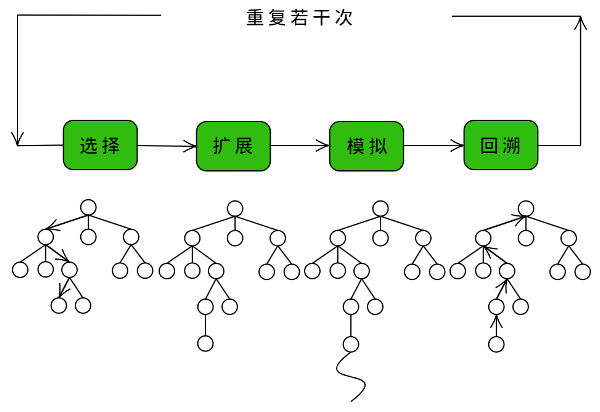
\includegraphics[width=0.6\textwidth]{fig/MCTS.png}
    \end{center}
    \caption{MCTS的四个阶段}\label{fig:1}
  \end{figure}

\end{frame}

\begin{frame}{MCTS算法改进}

  受到\cite{manna2022learning}的启发,我们可以将 $2N$ 维空间中的点映射成一个球面上的 Voronoi 分割,
  但这种映射并不是一一对应的,所以将整个搜索过程分为两步,第一步是在 $2N$ 维空间中进行搜索,
  以搜索出最具潜力的构型,设其顶点数为 $M$ ,第二步是基于第一步找到的构型,在 $2M$ 维空间中继续搜索,
  以搜索出此构型的最优形状. 

  为了保留树的特点,在扩展阶段,我们在以中心为根、半径为 $r\times 0.8^d$ 的超球面内随机生成一个点为新子节点,
  其中 $d$ 为根节点的深度. 同时,在随机的时候为了避免维度爆炸,
  我们先以根节点 $root$ 为中心随机出一个单位向量 $\vec\alpha$ 作为方向,
  再在 $[0,r\times 0.8^d]$ 内随机一个距离 $x$,
  则得到的新节点即为 $root+\vec\alpha$ ,保证了生成新节点时的随机性. 

\end{frame}

\begin{frame}{MCTS算法改进}

  另外,由于模拟阶段是为了给棋类游戏等问题中每个节点提供一个量化方法,
  而在本问题中,每个节点的好坏比较好量化,所以为了更好的适配此问题,我们去掉了模拟这一步骤,
  每个节点的好坏直接用该节点所代表的分割的目标函数来表示即可. 

  最后,由于各块面积相等的条件不好限制,我们将各块面积的方差也加入了目标函数,并且总周长和方差的尺度不同,
  所以在方差前再加入一个平衡系数来平衡两个量,于是最后的目标函数即为:
  $$\sum_{i=1}^Nl(\partial\Omega_i)+\lambda\mathrm{Var}(\{\mu(\Omega_i)\}).$$

\end{frame}

\section{实验与结果展示}

\begin{frame}{实验与结果展示}

  \textbf{实验设置}

  为验证改进后MCTS算法的有效性,实验针对球面等面积划分问题($n\leq 32$ )展开.
  算法参数设置为:两次MCTS的迭代次数上限分别为 $3\times 10^5$ 和 $0.5\times 10^5$,
  探索系数分别为 $c=50$ 和 $c=500$,平衡系数分别为 $\lambda=2$ 和 $\lambda=20$,
  搜索半径随节点深度按 $r=0.8^d$ 动态衰减.对比样例选用\cite{cox2010minimal}中给出的可能的最优结果. 

\end{frame}

\begin{frame}{实验与结果展示}

  \textbf{结果展示}

  \vspace{-0.3cm}

  \begin{figure}[ht]
    \centering
  
    % 第一行:三张子图
    \begin{subfigure}[b]{0.2\textwidth}
      \centering
      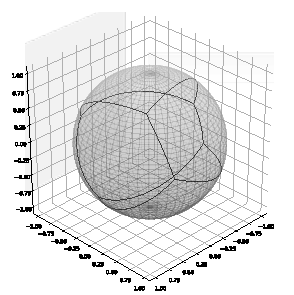
\includegraphics[width=\linewidth]{fig/1.pdf}
      \label{subfig:1}
    \end{subfigure}
    \hfill
    \begin{subfigure}[b]{0.2\textwidth}
      \centering
      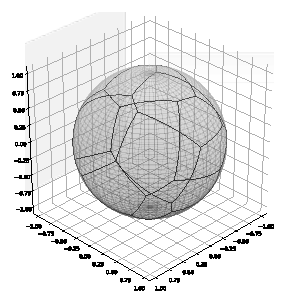
\includegraphics[width=\linewidth]{fig/2.pdf}
      \label{subfig:2}
    \end{subfigure}
    \hfill
    \begin{subfigure}[b]{0.2\textwidth}
      \centering
      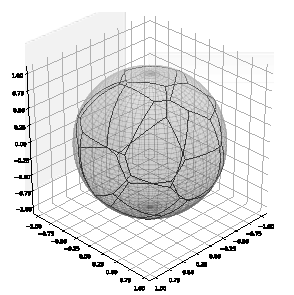
\includegraphics[width=\linewidth]{fig/3.pdf}
      \label{subfig:3}
    \end{subfigure}

    \vspace{-0.7cm}
  
    % 第二行:两张子图
    \begin{subfigure}[b]{0.2\textwidth}
      \centering
      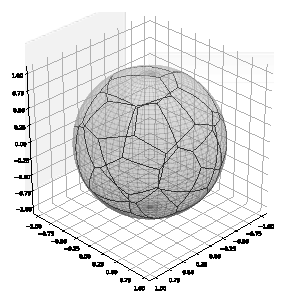
\includegraphics[width=\linewidth]{fig/4.pdf}
      \label{subfig:4}
    \end{subfigure}
    \hfill
    \begin{subfigure}[b]{0.2\textwidth}
      \centering
      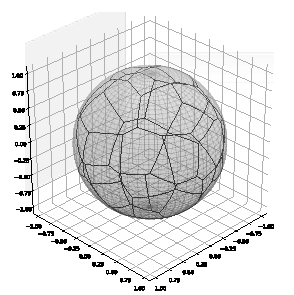
\includegraphics[width=\linewidth]{fig/5.pdf}
      \label{subfig:5}
    \end{subfigure}
  
    \caption{$n=5,13,20,25,32$ 时的球面等面积划分结果}
    \label{fig:sub}
  \end{figure}

\end{frame}

\section{结论与展望}

\begin{frame}{结论与展望}

  \textbf{结论}

  由图\ref{fig:sub}可以看出当 $n$ 较小时,利用改进后的MCTS算法能准确的找出最优解的构型,
  并且所求出的最小周长也与\cite{cox2010minimal}中给出的可能的最优结果非常接近;而在 $n$ 稍大时,
  MCTS算法也能较能准确的找出最优解的构型,同时所求出的最小周长也与\cite{cox2010minimal}中的结果接近;
  在 $n$ 较大时,MCTS算法求出的构型与\cite{cox2010minimal}中给出的较为接近,但求出的最小周长也比较接近. 

  \textbf{不足之处及未来展望}

  改进过后的MCTS搜索出来的结果并没有很完美,还是有许多地方需要改进的. 

  \begin{itemize}

    \item 还需要寻找更好的超参数,算法中各种参数的设置对于MCTS的收敛速度以及效果非常重要;
    \item 球面等面积划分问题有着明显但较为复杂的对称性,研究出该对称性也能在很大程度上提高搜索的效率,
    对搜索的精度也会有一定程度的提升;
    \item 还可以将神经网络加入到MCTS中,加速整个搜索过程,使得搜索结果更加精确。

  \end{itemize}

\end{frame}

\section{参考文献}

\begin{frame}{参考文献}
  
  \printbibliography[heading=none]

\end{frame}

\begin{frame}{Acknowledgement}

  \begin{center}

    \textcolor{gray}{\Huge{\centerline{\calligra{Thank you!}}}}

  \end{center}

\end{frame}

\end{document}
